\documentclass[9pt]{beamer}

% Use roboto Font (recommended)
\usepackage[sfdefault]{roboto}
%\usepackage[utf8]{inputenc}
%\usepackage[T1]{fontenc}
\usepackage[english]{babel}

% Define where theme files are located. ('/styles')
\usepackage{../flux-beamer-theme/styles/fluxmacros}
\usefolder{../flux-beamer-theme/styles}
% Use Flux theme v0.1 beta
% Available style: asphalt, blue, red, green, gray 
\usetheme[style=asphalt]{flux}

% Extra packages for the demo:
\usepackage{booktabs}
\usepackage{colortbl}
\usepackage{ragged2e}
\usepackage{schemabloc}

\usepackage{xcolor}

\newcommand{\mascot}{../graphics/tux.png}

% Informations
\title{\#AdoptYourOwnPenguin}
\subtitle{Linux Install Party}
\author{Christoph Großmann \& Lea Laux}
\institute{Ministry of Silly Walks}
\date{\today}
\titlegraphic{\mascot}

\newsavebox\mascotbox

\begin{lrbox}\mascotbox
	\includegraphics[height=3cm]{\mascot}%
\end{lrbox}

\definecolor{background-local}{named}{background}
%\definecolor{Gray-local}{HTML}{858b8f}
%\definecolor{text-local}{HTML}{4F5D66}
%\definecolor{primaryLight-local}{HTML}{34495e}
%\definecolor{primary-local}{HTML}{2d3e50}
%\definecolor{secondary-local}{HTML}{d15306}
%\definecolor{tertiary-local}{HTML}{35837b}

\newcommand{\DarkBG}{\definecolor{background}{named}{primaryLight}}
\newcommand{\ResetBG}{\definecolor{background}{named}{background-local}}

\newcommand{\sectionframe}[1]{%
\DarkBG%
\begin{frame}[plain]%
\section{#1}\centering\Huge\color{background-local}\textbf{#1}%
\vfill\usebox\mascotbox%
\end{frame}%
\ResetBG%
}

\usepackage[most]{tcolorbox}

\tcbset	{
		frame code={}
		center title,
		left=0pt,
		right=0pt,
		top=0pt,
		bottom=0pt,
		colback=primaryLight,
		colframe=white,
		width=.9\linewidth,
		enlarge left by=0mm,
		boxsep=5pt,
		arc=1pt,outer arc=0pt,
		%height=2\baselineskip
		}

\newcommand{\bash}[1]{\begin{tcolorbox}\color{background-local}> \textbf{#1}\end{tcolorbox}}

\begin{document}

	\titlepage
	
	\begin{frame}
	\frametitle{Table of contents}
	\tableofcontents
\end{frame}

	
	\sectionframe{Introduction to Linux}
	\begin{frame}
	\frametitle{Some information about Linux}
	\subsection{Some information about Linux}
	
	\begin{itemize}
		\item Operating systems based on the Linux kernel\cite{linux}
		\item The Linux kernel is part of the UNIX family
		\item (Mostly) open source
		\item Fit for a range of different use cases:
			\begin{tiny}
				\begin{itemize}
					\item Desctop computers
					\item Server
					\item Smartphones
					\item TVs
					\item Tablets
					\item IoT devices
					\item $\dots$
				\end{itemize}
			\end{tiny}
		\item Around since the mid-1990s
		\item Many of the supporting system software and libraries are provided by the GNU project\cite{gnu}
	\end{itemize}
\end{frame}

	\begin{frame}
	\frametitle{Advantages of Linux}
	\subsection{Advantages of Linux}
	
	\begin{itemize}
		\item Free
		\item Open source
			\begin{tiny}
				\begin{itemize}
					\item Freedom to run the program for whatever purpose
					\item Freedom to redistribute copies of the program
					\item Freedom to study the inner workings of the program
					\item Freedom to make changes to the program
					\item Freedom to distribute copies of the modified versions
				\end{itemize}
			\end{tiny}
		\item A system under your exclusive control
		\item Multi-purpose
		\item Extremely customisable
		\item Package managers
		\item Fewer viruses and malware
		\item $\dots$
	\end{itemize}

	\vfill
	
	There are some closed source programs. Most distributions give you the option whether or not to use them. Furthermore there are some paid for Linux distributions but they mainly come into play for server operating systems.
\end{frame}

	\begin{frame}
	\frametitle{The pieces of a Linux operating system}
	\subsection{The pieces of a Linux operating system}
	
	\begin{enumerate}
		\item \textbf{Bootloader}:\\ The software managing the boot process of your computer and thus responsible for starting the operating system.
		\item \textbf{Kernel}:\\ The actual Linux. It manages the CPU, the memory and all peripheral devices.
		\item \textbf{Init system}:\\ Bootstraps the user space and controls the daemons. Takes over after the bootloader is done.
		\item \textbf{Daemons}:\\ Background services like printing, sound, or scheduling.
		\item \textbf{Graphical Server}:\\ Renders and displays all graphics.
		\item \textbf{Desktop environment}:\\ The piece the user interacts with. There are a few different environments to choose from (GNOME, KDE, Mate, XFCE, etc.).
		\item \textbf{Applications}:\\ Software that is not included with any of the previous pieces. Can be installed via a package manager or by hand.
	\end{enumerate}
\end{frame}

	\begin{frame}
	\frametitle{Linux distributions}
	\subsection{Linux distributions}
	
	\begin{columns}
		\begin{column}{.25\linewidth}
			\begin{block}{Well known distros:}
				\begin{itemize}
					\item Debian
					\item Ubuntu
					\item Arch Linux
					\item Manjaro
					\item openSuse
					\item Red Hat
					\item Fedora
					\item Kali
					\item Linux Mint
					\item $\dots$
				\end{itemize}
			\end{block}
		\end{column}
		\hfill
		\begin{column}{.7\linewidth}
			\begin{figure}
				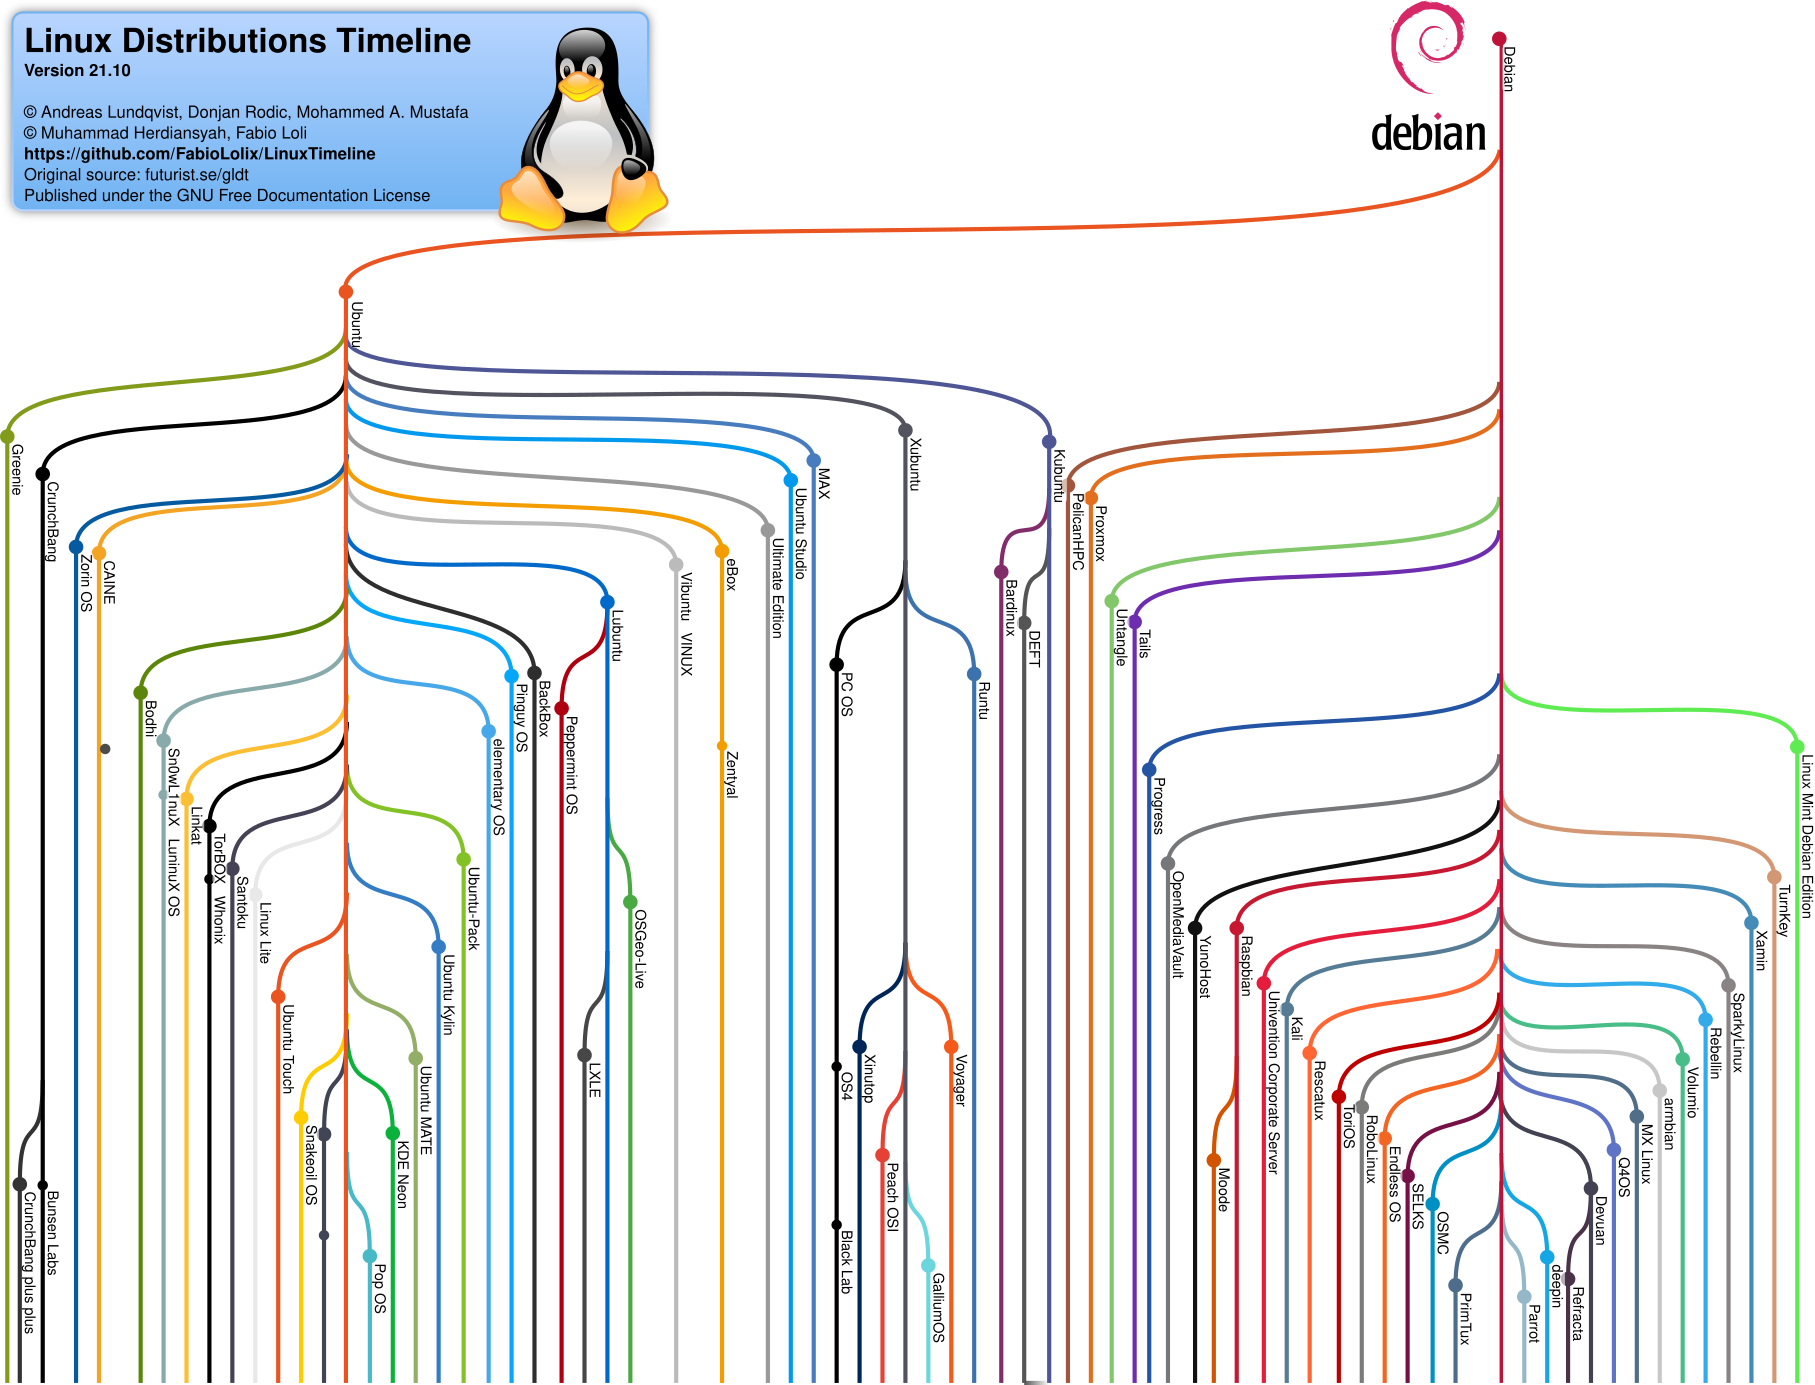
\includegraphics[width=\linewidth]{../graphics/debian_distro_timeline/debian_distro_timeline.png}
				\caption{Excerpt from the Linux distro tree for Debian \cite{distrograph}}
			\end{figure}
		\end{column}
	\end{columns}
	
	\vfill
	
	\centering
	See DistroWatch\cite{distrowatch} for a comprehensive list of all Linux distributions.
\end{frame}

	
	\sectionframe{A selection of noteworthy distributions}
	\begin{frame}
	\frametitle{Debian}
	\subsection{Debian}
	
	\vfill
	\begin{columns}
		\begin{column}{.65\linewidth}
			\begin{itemize}
				\item Around since 1993
				\item Comes with over 50,000 packages
				\item Supported desktop environments:
					\begin{tiny}
						\begin{itemize}
							\item XFCE
							\item GNOME
							\item KDE
							\item MATE
							\item Cinnamon
							\item LXDE
							\item MATE
						\end{itemize}
					\end{tiny}
				\item Release cycle
					\begin{itemize}
						\item A stable version is released every 2 years
						\item Each version will receive updates for 3 years
						\item Those updates will only contain security updates and fixes
						\item After that the version will receive security updates for 2 more years
						\item oldoldstable – oldstable – \textbf{stable} – testing
						– unstable – experimental
					\end{itemize}
				\item Package manager: \texttt{dpkg} / \texttt{apt}
			\end{itemize}
		\end{column}
		\hfill
		\begin{column}{.34\linewidth}
			
\includegraphics[width=\linewidth]{../graphics/logos/Debian/openlogo.png}
		\end{column}
	\end{columns}
	\vfill
\end{frame}

	\begin{frame}
	\frametitle{Ubuntu and Linux Mint}
	\subsection{Ubuntu and Linux Mint}
	
	\begin{columns}
		\begin{column}[t]{.45\linewidth}
			\begin{block}{Ubuntu}
				\begin{itemize}
					\item Around since 2004
					\item Derivative of Debian
					\item Very new-user-friendly
					\item Default desktop: GNOME
					\item Packages are based on packages from Debian's unstable branch
					\item Release cycle
						\begin{itemize}
							\item New version every 6 months
							\item Long-term support version every 2 years
							\item LTS version updates for 5 years
						\end{itemize}
					\item Package manager: \texttt{apt}
				\end{itemize}
			\end{block}
		\end{column}
		\hfill
		\begin{column}[t]{.45\linewidth}
			\begin{block}{Linux Mint}
				\begin{itemize}
					\item Around since 2006
					\item Derivative of Ubuntu
					\item Also very new-user-friendly
					\item Default desktop: Cinnamon / MATE / Xfce
					\item Full out-of-the-box multimedia support
					\item Release cycle same as Ubuntu
					\item Package manager: \textit{dpkg} / \textit{Flatpak} / \texttt{apt}
				\end{itemize}
			\end{block}
		\end{column}
	\end{columns}
	
	\vfill
	
	\begin{columns}
		\begin{column}{.5\linewidth}
			\centering
\includegraphics[height=3\baselineskip]{../graphics/logos/Ubuntu/ubuntu-logo-2022.png}
		\end{column}
		\hfill
		\begin{column}{.5\linewidth}
			\centering
\includegraphics[height=3\baselineskip]{../graphics/logos/Mint/leaf.png}
		\end{column}
	\end{columns}
\end{frame}

	\begin{frame}
	\frametitle{Arch Linux and Manjaro}
	\subsection{Arch Linux and Manjaro}
	
	\begin{columns}
		\begin{column}[t]{.45\linewidth}
			\begin{block}{Arch Linux}
				\begin{itemize}
					\item Around since 2002
					\item Release cycle:
						\begin{itemize}
							\item Rolling release model
							\item Latest stable versions of most software
							\item \textbf{stable} – testing – unstable
							\item Quick access to new versions of software
						\end{itemize}
					\item Package manager: \texttt{pacman}
					\item Additional package repository called \textbf{A}rch \textbf{U}ser \textbf{R}epository
					\item Get the package manager \texttt{yay} if you can
					\item No visual installation!
				\end{itemize}
			\end{block}
		\end{column}
		\hfill
		\begin{column}[t]{.45\linewidth}
			\begin{block}{Manjaro}
				\begin{itemize}
					\item Around since 2011
					\item Derivative of Arch Linux
					\item Default desktop: Xfce / KDE Plasma / GNOME / Phosh
					\item Focus on user-friendliness and accessibility
					\item Still most of the benefits of Arch
					\item Visual installer
					\item Uses the same package repositories as Arch
					\item Package manager: \texttt{pacman}
				\end{itemize}
			\end{block}
		\end{column}
	\end{columns}

	
	
	\vfill
	
	\begin{columns}
		\begin{column}{.5\linewidth}
			\centering
\includegraphics[height=3\baselineskip]{../graphics/logos/Arch/archlinux-logo-dark-1200dpi.b42bd35d5916.png}
		\end{column}
		\hfill
		\begin{column}{.5\linewidth}
			\centering
\includegraphics[height=2\baselineskip]{../graphics/logos/Manjaro/Main_page_logo.png}
		\end{column}
	\end{columns}
\end{frame}

	
	\sectionframe{Desktop environments}
	\begin{frame}
	\frametitle{Some information about Linux}
	\subsection{Some information about Linux}
	
	\begin{itemize}
		\item Operating systems based on the Linux kernel\cite{linux}
		\item The Linux kernel is part of the UNIX family
		\item (Mostly) open source
		\item Fit for a range of different use cases:
			\begin{tiny}
				\begin{itemize}
					\item Desctop computers
					\item Server
					\item Smartphones
					\item TVs
					\item Tablets
					\item IoT devices
					\item $\dots$
				\end{itemize}
			\end{tiny}
		\item Around since the mid-1990s
		\item Many of the supporting system software and libraries are provided by the GNU project\cite{gnu}
	\end{itemize}
\end{frame}

	\subsection{KDE, MATE, GNOME, Cinnamon, Xfce, Budgie, LXQt, and Deepin}
	\begin{frame}
	\frametitle{KDE Plasma desktop environment}
	
	\begin{center}
		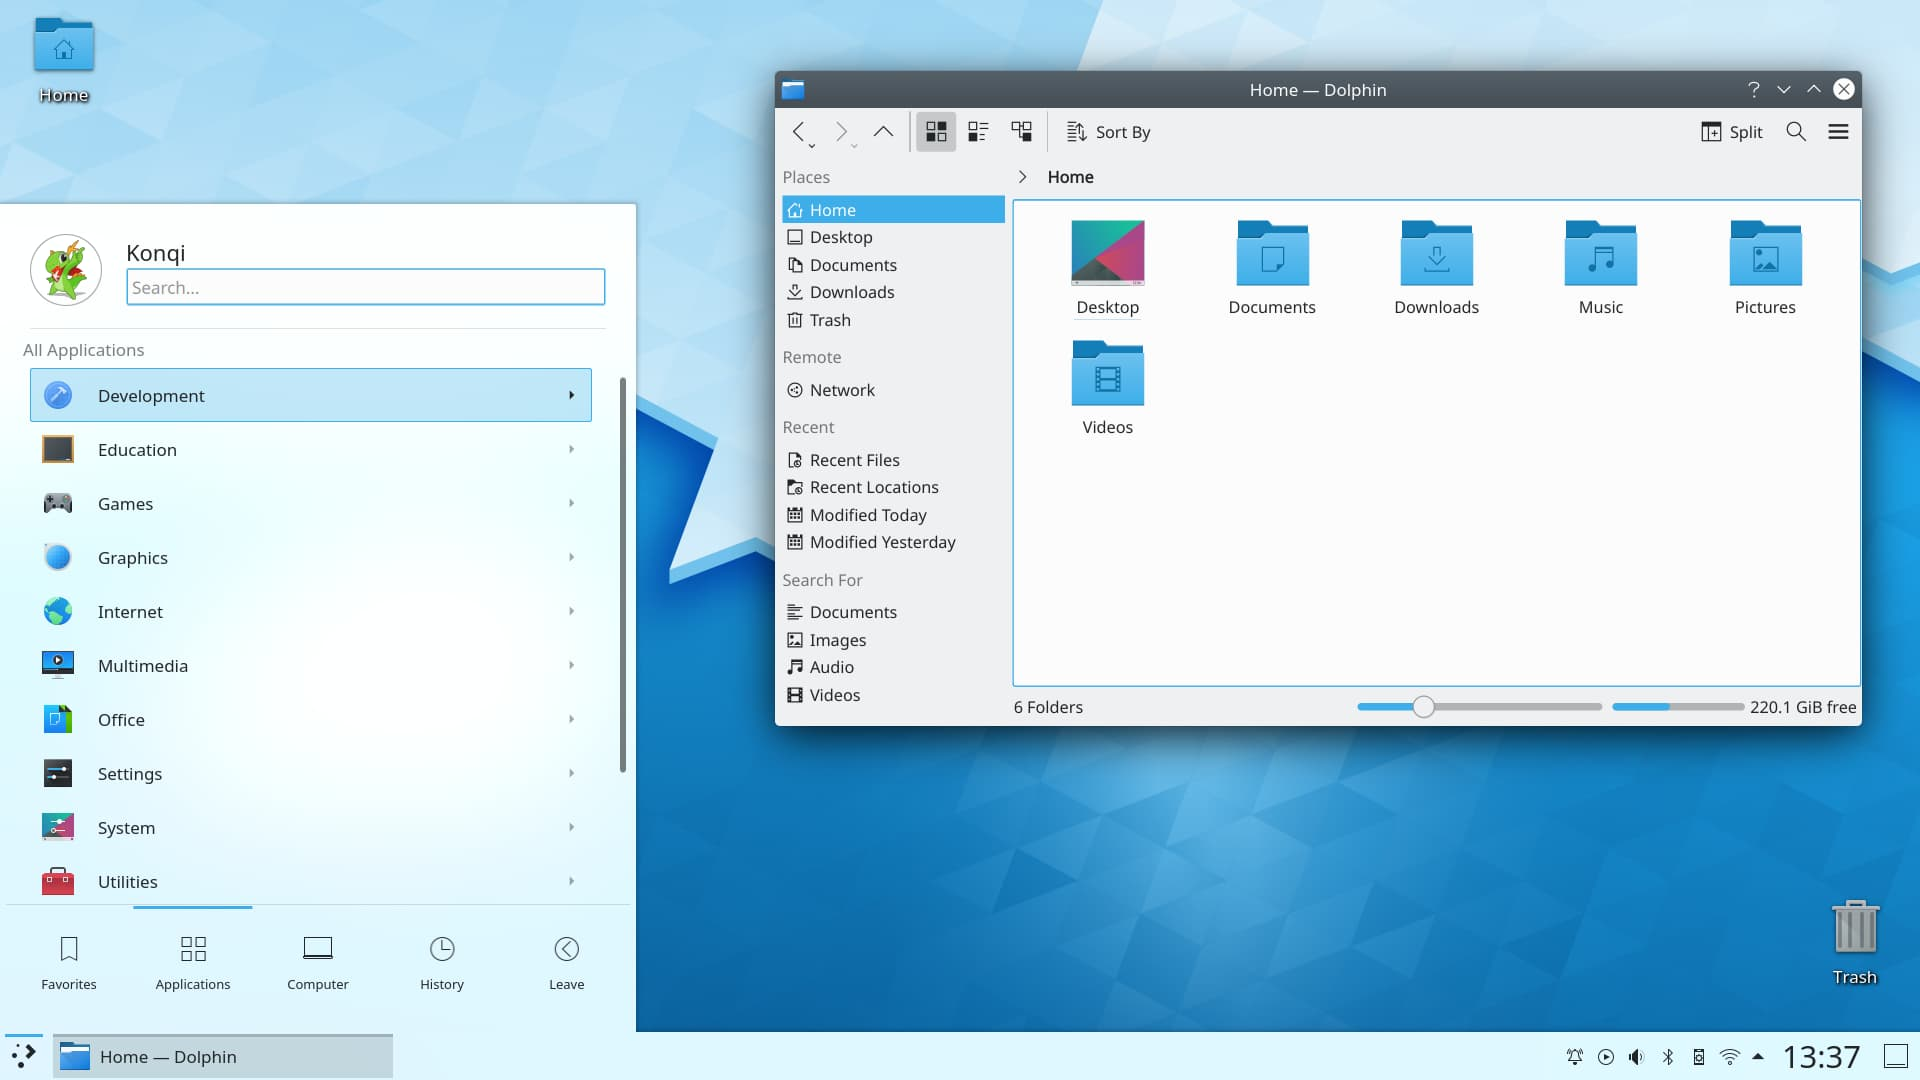
\includegraphics[width=.7\linewidth]{../graphics/desktop_examples/kde.jpg}
	\end{center}%

	\vspace{-\baselineskip}
	
	\begin{columns}
		\begin{column}[t]{.7\linewidth}
			\begin{exampleblock}{Advantages:}
				\begin{itemize}
					\item Highly customisable
					\item KDE Connect (connect your phone to the computer)
					\item Modern and polished user interface
					\item Several useful tools built-in
				\end{itemize}
			\end{exampleblock}
		\end{column}
		\hfill
		\begin{column}[t]{.28\linewidth}
			\begin{alertblock}{Disadvantages:}
				\begin{itemize}
					\item Customization options can be overwhelming
					\item Not suitable for older computers
				\end{itemize}
			\end{alertblock}
		\end{column}
	\end{columns}
	\hfill
\end{frame}

	\begin{frame}
	\frametitle{MATE desktop environment}
	
	\begin{center}
		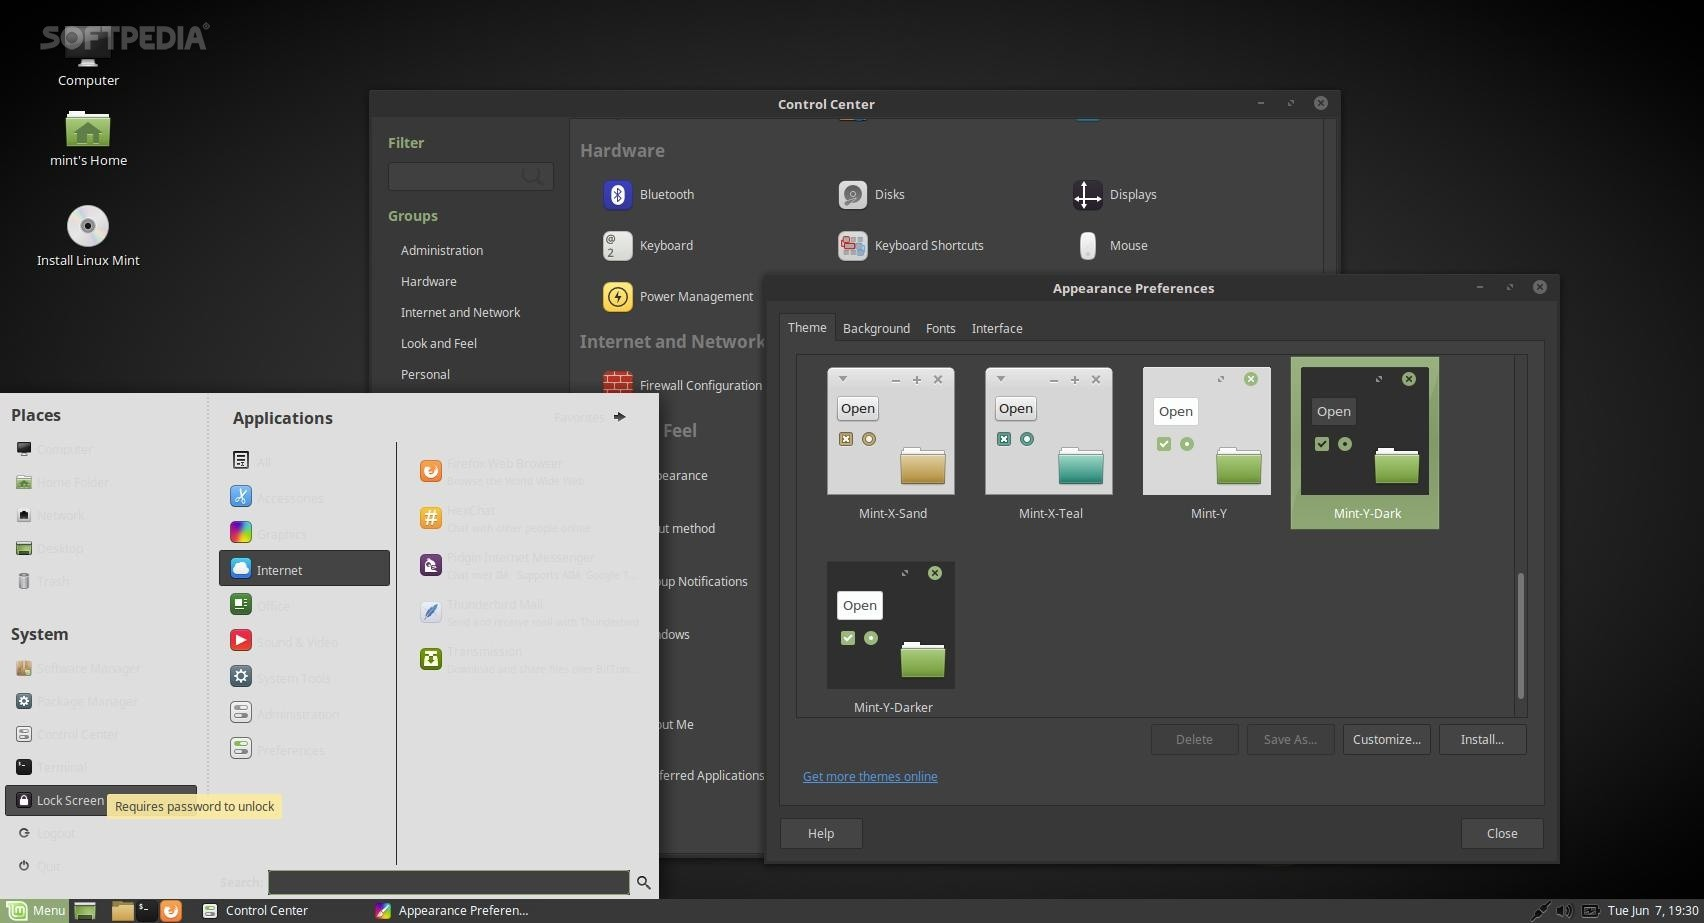
\includegraphics[width=.7\linewidth]{../graphics/desktop_examples/mate.jpg}
	\end{center}%
	
	\vspace{-\baselineskip}
	
	\begin{columns}
		\begin{column}[t]{.7\linewidth}
			\begin{exampleblock}{Advantages:}
				\begin{itemize}
					\item Suitable for almost everyone
					\item Easy to use, robust experience, and lightweight
					\item Simple yet Customizable
					\item Collection of basic applications and built-in useful tools
				\end{itemize}
			\end{exampleblock}
		\end{column}
		\hfill
		\begin{column}[t]{.28\linewidth}
			\begin{alertblock}{Disadvantages:}
				\begin{itemize}
					\item Does not offer the most intuitive user experience
					\item Not that modern-looking
				\end{itemize}
			\end{alertblock}
		\end{column}
	\end{columns}
	\hfill
\end{frame}

	\begin{frame}
	\frametitle{GNOME desktop environment}
	
	\begin{center}
		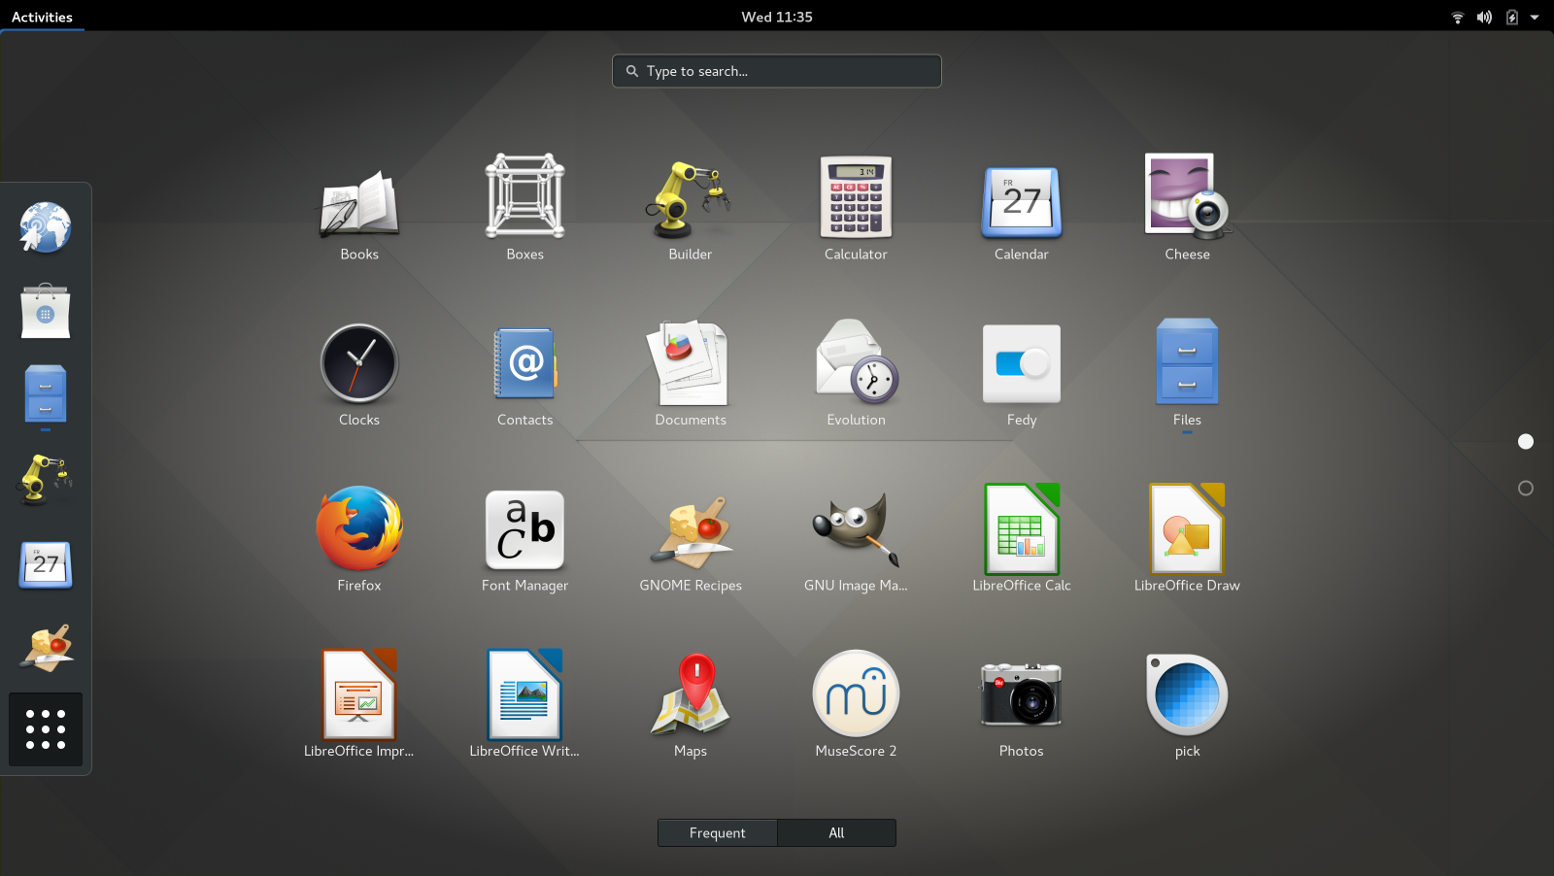
\includegraphics[width=.7\linewidth]{../graphics/desktop_examples/gnome.png}
	\end{center}%
	
	\vspace{-\baselineskip}
	
	\begin{columns}
		\begin{column}[t]{.7\linewidth}
			\begin{exampleblock}{Advantages:}
				\begin{itemize}
					\item Easy to use and customizable
					\item Modern and touch-friendly UI
					\item User interface aims to provide a unique experience
					\item Can extend functionalities with GNOME Shell Extensions
				\end{itemize}
			\end{exampleblock}
		\end{column}
		\hfill
		\begin{column}[t]{.28\linewidth}
			\begin{alertblock}{Disadvantages:}
				\begin{itemize}
					\item Not suitable for older computers
					\item User Interface isn’t tailored for a Windows user
				\end{itemize}
			\end{alertblock}
		\end{column}
	\end{columns}
	\hfill
\end{frame}

	\begin{frame}
	\frametitle{Cinnamon desktop environment}
	
	\begin{center}
		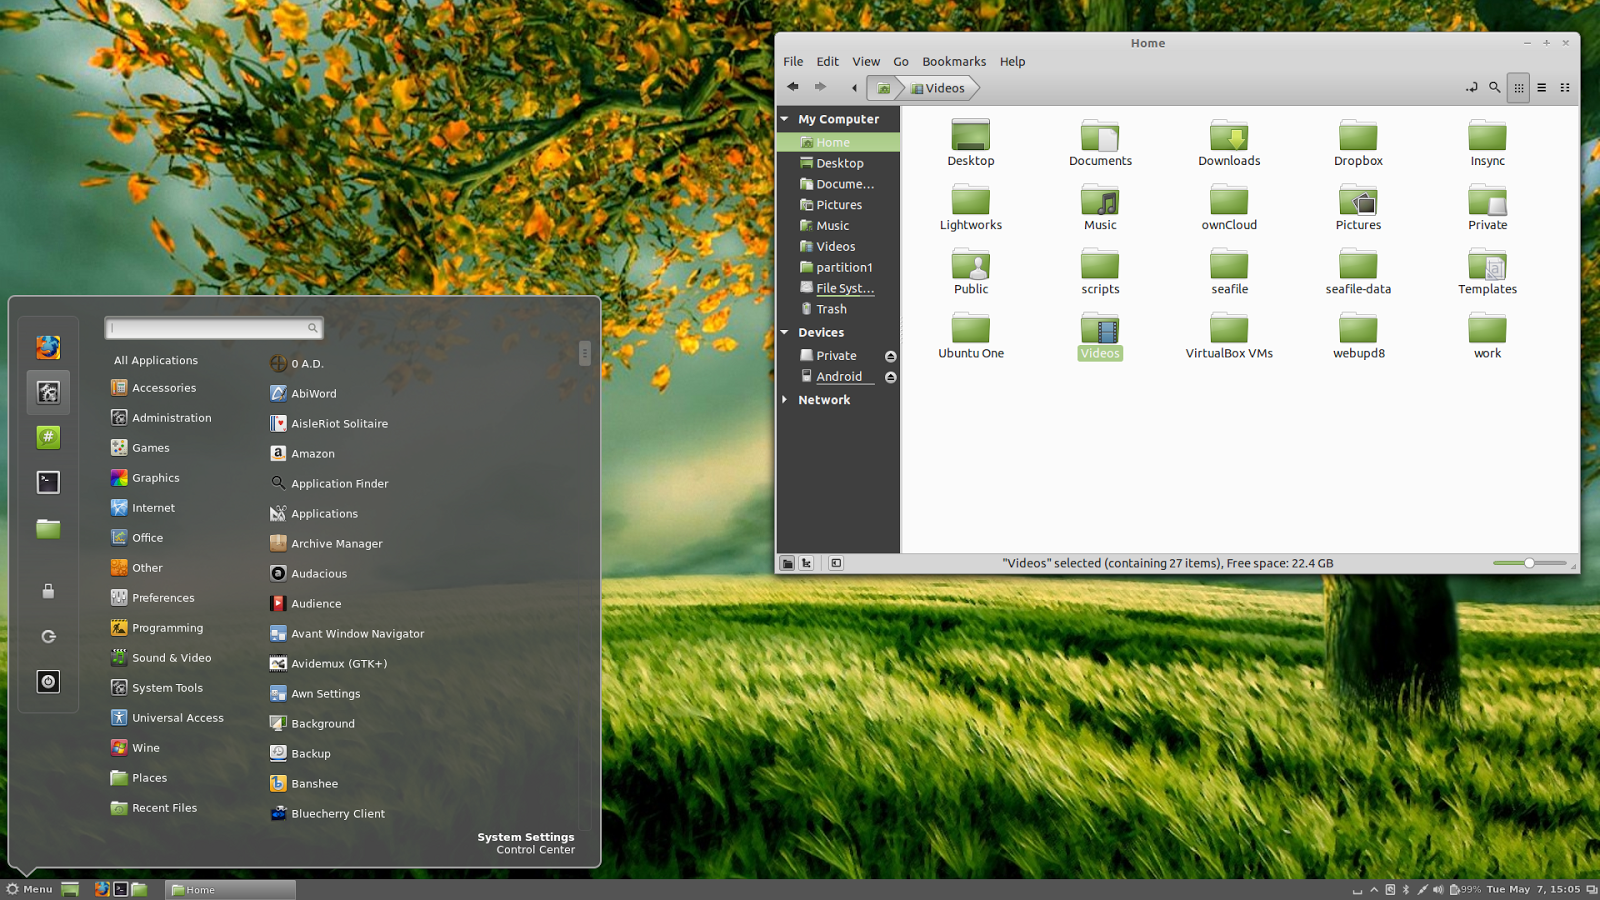
\includegraphics[width=.7\linewidth]{../graphics/desktop_examples/cinnamon.png}
	\end{center}%
	
	\vspace{-\baselineskip}
	
	\begin{columns}
		\begin{column}[t]{.7\linewidth}
			\begin{exampleblock}{Advantages:}
				\begin{itemize}
					\item Default desktop environment for Linux Mint
					\item Similar to the Windows user interface
					\item Sleek and polished look
					\item Pretty customizable
				\end{itemize}
			\end{exampleblock}
		\end{column}
		\hfill
		\begin{column}[t]{.28\linewidth}
			\begin{alertblock}{Disadvantages:}
				\begin{itemize}
					\item Does not offer the most intuitive user experience
					\item Not that modern-looking
				\end{itemize}
			\end{alertblock}
		\end{column}
	\end{columns}
	\hfill
\end{frame}

	\begin{frame}
	\frametitle{Xfce Plasma desktop environment}
	
	\begin{center}
		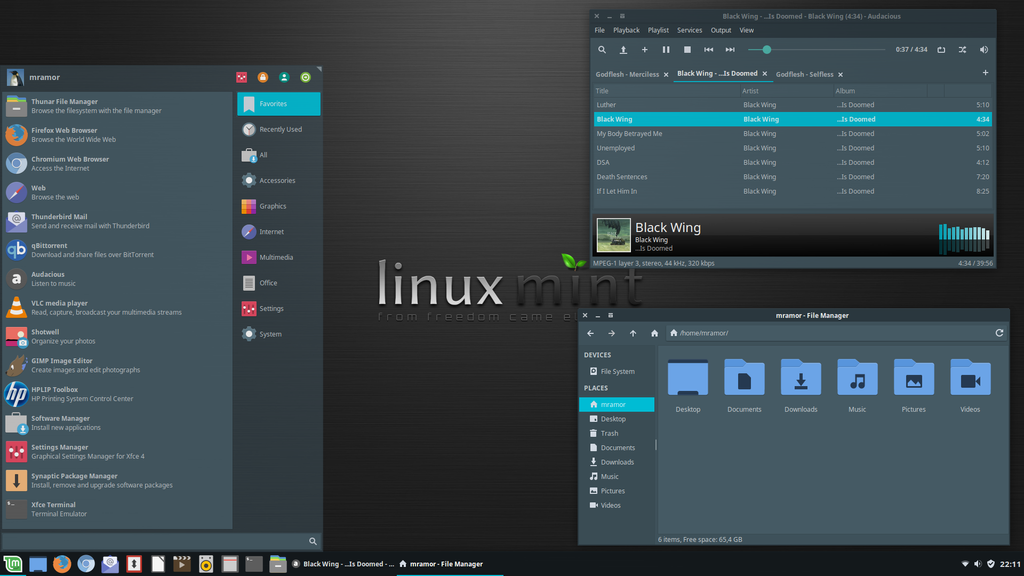
\includegraphics[width=.7\linewidth]{../graphics/desktop_examples/xfce.png}
	\end{center}%
	
	\vspace{-\baselineskip}
	
	\begin{columns}
		\begin{column}[t]{.7\linewidth}
			\begin{exampleblock}{Advantages:}
				\begin{itemize}
					\item Lightweight and adaptable to old hardware
					\item Modern and visually appealing
					\item Windows-like familiar UI
					\item Feature-rich user experience
				\end{itemize}
			\end{exampleblock}
		\end{column}
		\hfill
		\begin{column}[t]{.28\linewidth}
			\begin{alertblock}{Disadvantages:}
				\begin{itemize}
					\item No advanced customizations
					\item User experience could be better
				\end{itemize}
			\end{alertblock}
		\end{column}
	\end{columns}
	\hfill
\end{frame}

	\begin{frame}
	\frametitle{Budgie desktop environment}
	
	\begin{center}
		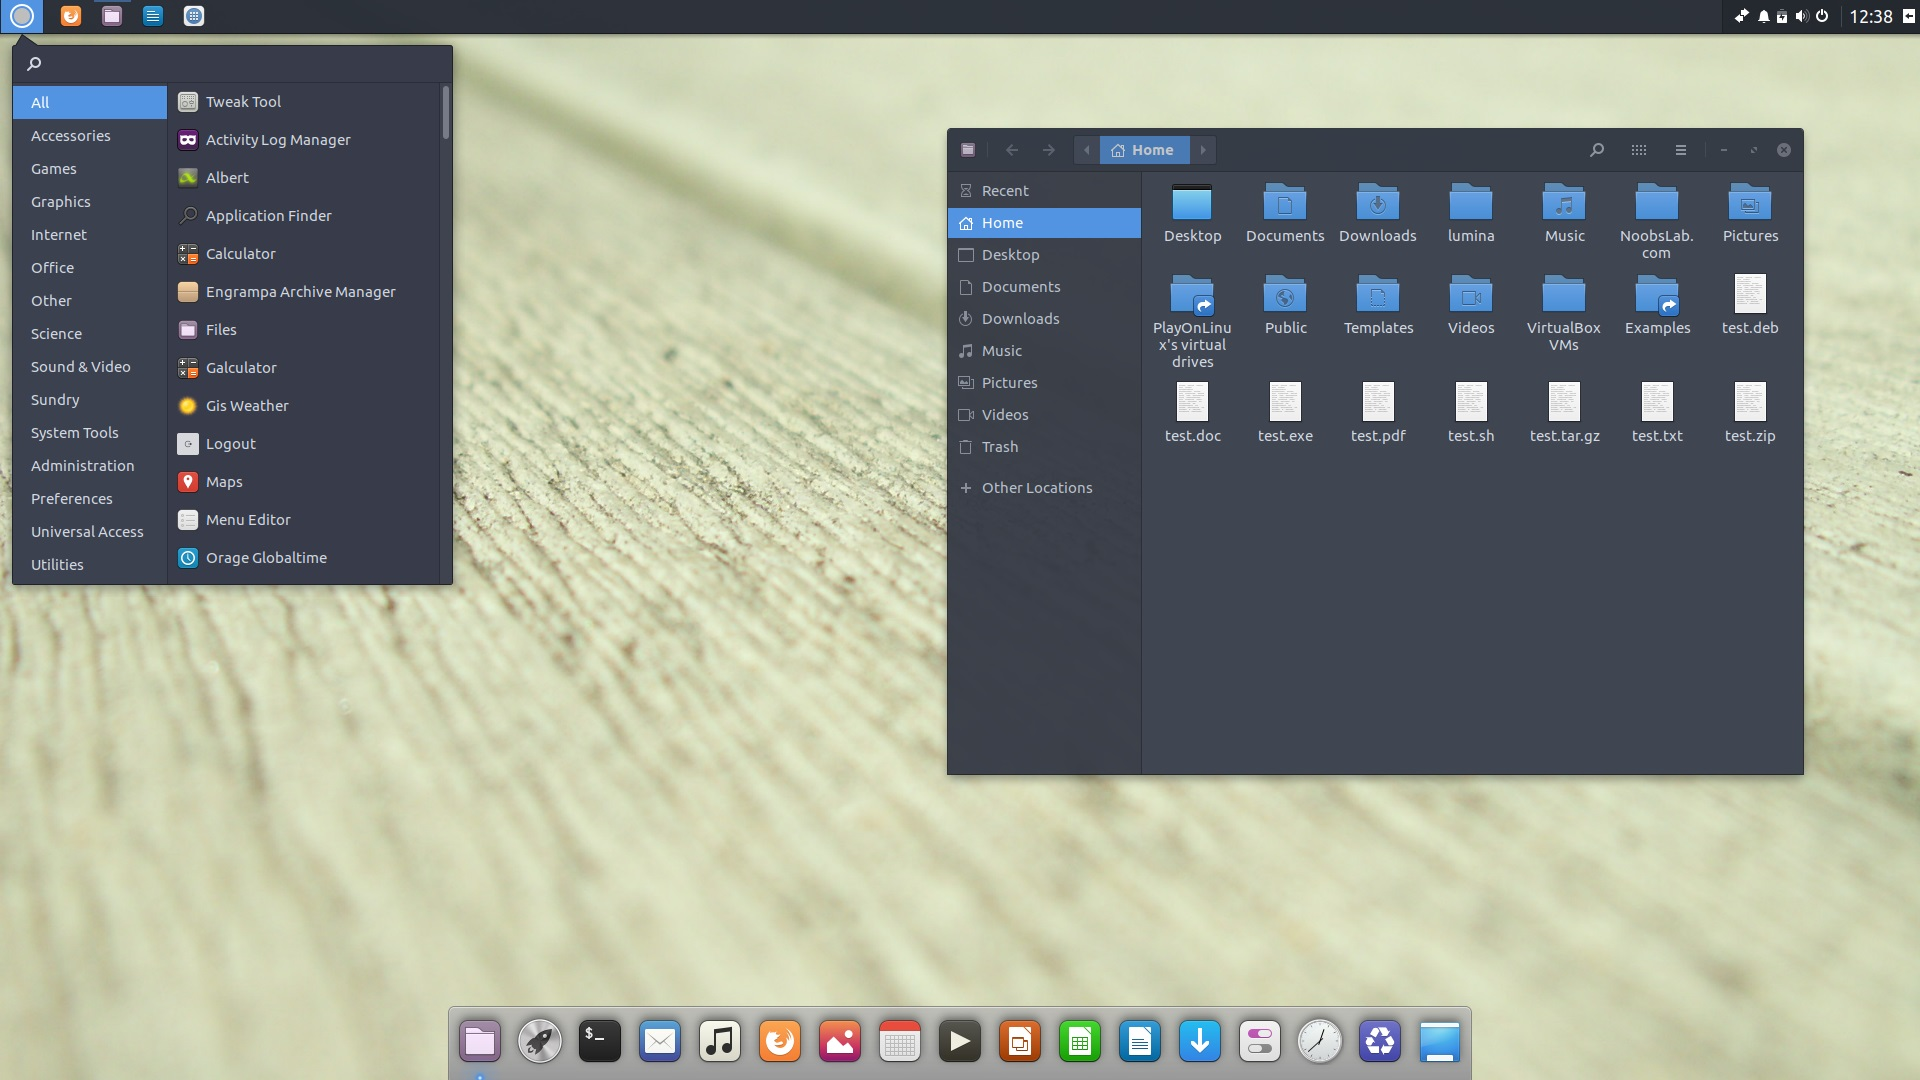
\includegraphics[width=.7\linewidth]{../graphics/desktop_examples/budgie.jpg}
	\end{center}%
	
	\vspace{-\baselineskip}
	
	\begin{columns}
		\begin{column}[t]{.7\linewidth}
			\begin{exampleblock}{Advantages:}
				\begin{itemize}
					\item Solid and intuitive
					\item Modern UI and elegant looks
					\item Seamless desktop experience
					\item Mixed of modern UI and a traditional user interface
				\end{itemize}
			\end{exampleblock}
		\end{column}
		\hfill
		\begin{column}[t]{.28\linewidth}
			\begin{alertblock}{Disadvantages:}
				\begin{itemize}
					\item Not lightweight
					\item Available only on few distributions
				\end{itemize}
			\end{alertblock}
		\end{column}
	\end{columns}
	\hfill
\end{frame}

	\begin{frame}
	\frametitle{LXQt desktop environment}
	
	\begin{center}
		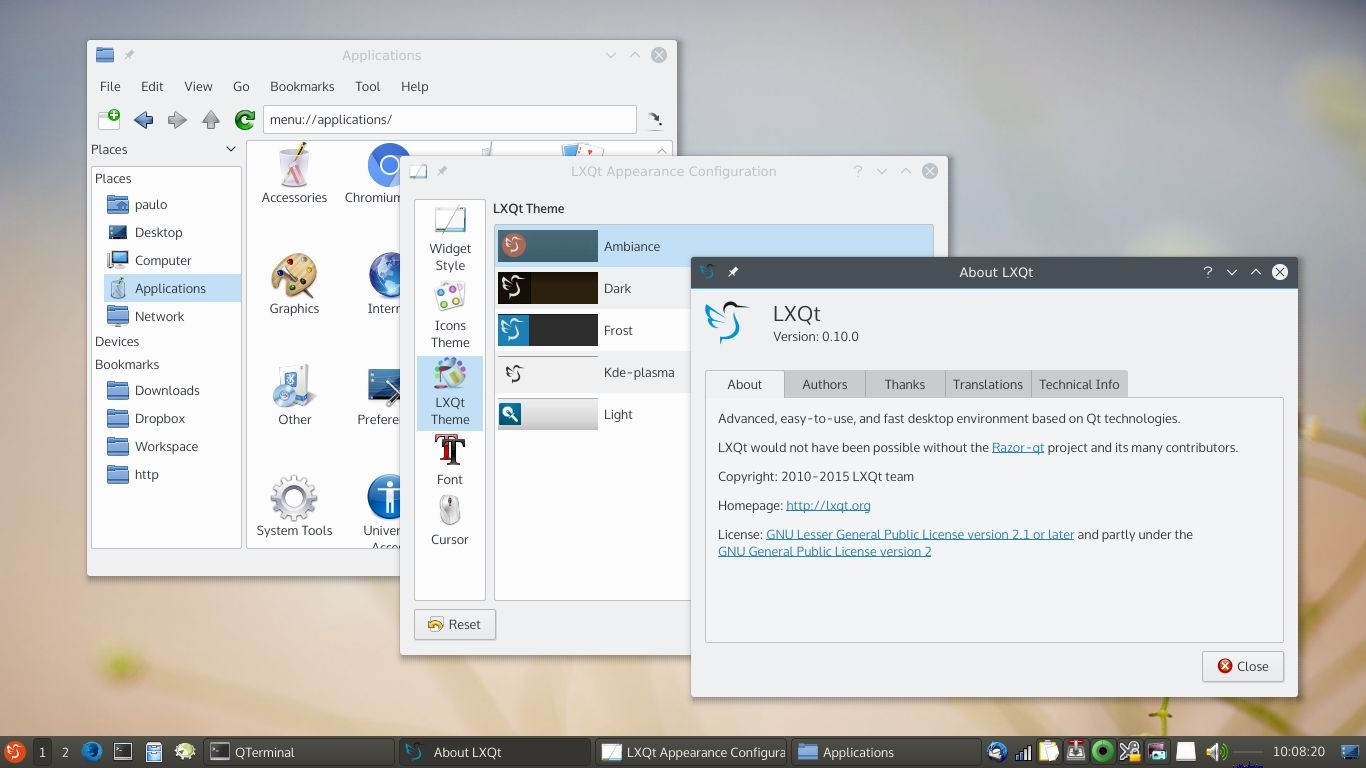
\includegraphics[width=.7\linewidth]{../graphics/desktop_examples/lxqt.jpg}
	\end{center}%
	
	\vspace{-\baselineskip}
	
	\begin{columns}
		\begin{column}[t]{.7\linewidth}
			\begin{exampleblock}{Advantages:}
				\begin{itemize}
					\item Extremely fast performing and lightweight
					\item Less resource consumption
					\item Decent UI for a lightweight desktop environment (else rather unappealing)
				\end{itemize}
			\end{exampleblock}
		\end{column}
		\hfill
		\begin{column}[t]{.28\linewidth}
			\begin{alertblock}{Disadvantages:}
				\begin{itemize}
					\item Not very customizable
					\item Available only on few distributions
				\end{itemize}
			\end{alertblock}
		\end{column}
	\end{columns}
	\hfill
\end{frame}

	\begin{frame}
	\frametitle{Deepin desktop environment}
	
	\begin{center}
		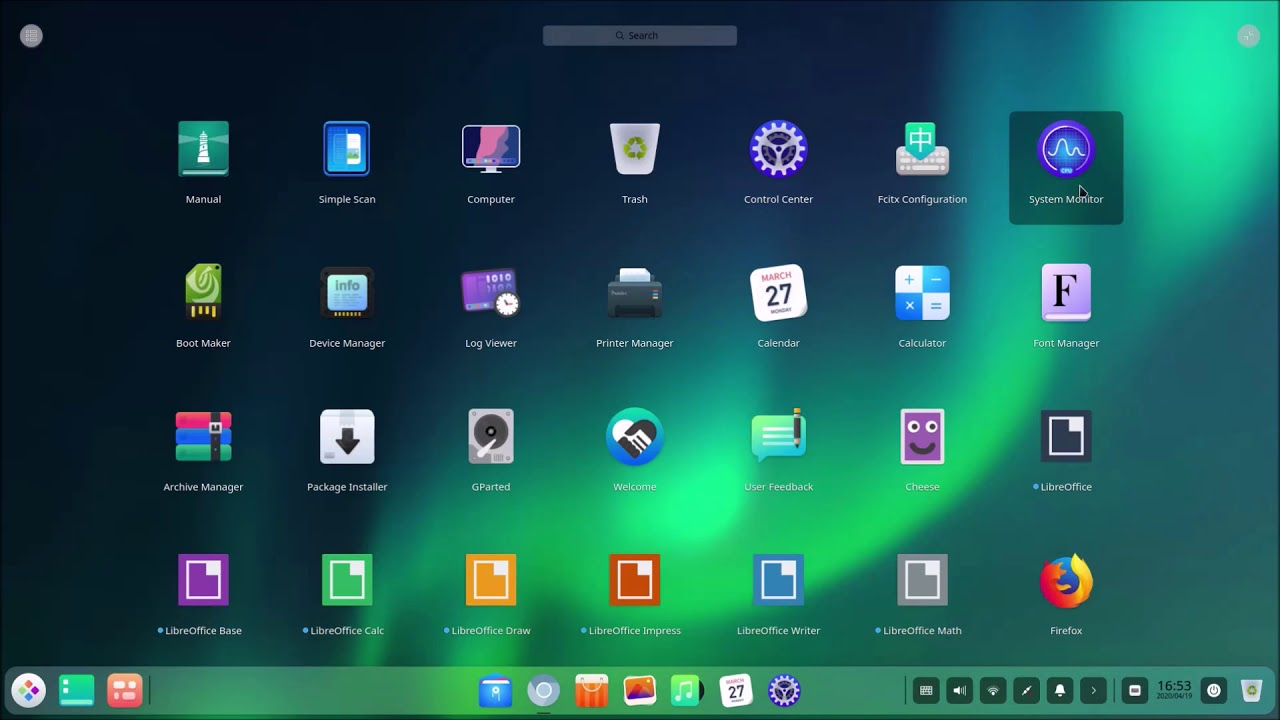
\includegraphics[width=.7\linewidth]{../graphics/desktop_examples/deepin.jpg}
	\end{center}%
	
	\vspace{-\baselineskip}
	
	\begin{columns}
		\begin{column}[t]{.7\linewidth}
			\begin{exampleblock}{Advantages:}
				\begin{itemize}
					\item Eye candy user interface
					\item Sleek animations
					\item Most beautiful macOS-like user interface
				\end{itemize}
			\end{exampleblock}
		\end{column}
		\hfill
		\begin{column}[t]{.28\linewidth}
			\begin{alertblock}{Disadvantages:}
				\begin{itemize}
					\item Heavy on resource usage 
					\item Sluggish at times
				\end{itemize}
			\end{alertblock}
		\end{column}
	\end{columns}
	\hfill
\end{frame}

	
	\sectionframe{Installing and working with a Linux system}
	\begin{frame}
	\frametitle{Linux installation}
	\subsection{Linux installation}
	
	\begin{enumerate}
		\item Choose the distro you want to install.
		\item Download the .iso-file you want.
		\item Write the .iso-file to USB-stick.
		\item Start your pc an enter the boot loader menu
		\item Boot using the USB-stick as boot medium.
		\item Go throw all installer steps and wait for the installation to finish.
		\item Well done, you've got yourself a Linux!
	\end{enumerate}
\end{frame}

	\begin{frame}
	\frametitle{Basics of your new Linux system}
	\subsection{Basics of your new Linux system}
	
	\begin{itemize}
		\item If you need superuser permissions to execute a command use \bash{sudo [command]}
		\item The log in as the superuser use the command \bash{su}
		\item Superuser permissions are needed to use your package manager.
		\item To get some information about a command use \bash{man [command]}
	\end{itemize}
\end{frame}

	\begin{frame}
	\frametitle{Installing and updating software}
	\subsection{Installing and updating software}
	
	bla, bla, bla, ...
\end{frame}

	\begin{frame}
	\frametitle{Troubleshooting}
	\subsection{Troubleshooting}
	
	\begin{exampleblock}{\textbf{Keep calm} ...}
		... and search for the origin of your error.
	\end{exampleblock}

	\vfill

	\begin{block}{Steps to take}
		\begin{itemize}
			\item Most likely someone else already had the same problem. So throw the information you've got about the error into a search machine of your choice.
			\item Wikis are a great source for help
			\begin{itemize}
				\item \url{https://wiki.ubuntuusers.de/}
				\item \url{https://wiki.archlinux.org/}
			\end{itemize}
			\item Mailing lists can also contain valuable information.
			\item Ask people you know with some knowledge of Linux.
			\item Only clear the cache of your package manager when you're sure everything works. You might need the older versions of packages stored there.
		\end{itemize}
	\end{block}

	\vfill

	\begin{alertblock}{And don't forget ...}
		... to make regular \textbf{backups}!
	\end{alertblock}
\end{frame}

	
	%\begin{frame}%[allowframebreaks]{References}
	\frametitle{List of figures}
	
	\listoffigures
\end{frame}

	\begin{frame}%[allowframebreaks]{References}
	\frametitle{References}
	\section{References}
	
	\nocite{*}
	\bibliography{adoptyourownpenguin_presentation.bib}
	\bibliographystyle{abbrv}
\end{frame}

	\begin{frame}
	\frametitle{Flux beamer theme}
	
	Flux is a modern style beamer presentation. It is provided as a work in progress version and may suffer from inconsistencies. Sources and complementary information are available at:\\[.2\baselineskip]
	\url{github.com/pvanberg/flux-beamer}\\
	
	\vfill
	
	Flux is licensed under GNU General Public License v3.\\[.2\baselineskip]
	\url{http://www.gnu.org/licenses}\\
	
	\vfill
	
	Flux is inspired by \textbf{Metropolis} theme from Matthias Vogelgesang:\\[.2\baselineskip]
	\url{https://github.com/matze/mtheme} 
	
\end{frame}

	\newcommand{\selfrefleftcolumn}{.75\linewidth}
\newcommand{\selfrefrightcolumn}{.2\linewidth}

\begin{frame}
	\frametitle{This presentation}
	
	\begin{columns}%
		\begin{column}{\selfrefleftcolumn}%
			The presentation can be found here:\\[.2\baselineskip]%
			\url{https://github.com/christoph-grossmann/AdoptYourOwnPenguin}%
		\end{column}%
		\hfill%
		\begin{column}{\selfrefrightcolumn}%
			
\includegraphics[width=\linewidth]{../graphics/repo_link_qr_code.png}%
		\end{column}%
	\end{columns}%
	
	\vfill%
	
	\begin{columns}%
		\begin{column}{\selfrefrightcolumn}%
			
\includegraphics[width=\linewidth]{../graphics/lea_laux_presentation_qr_code.png}%
		\end{column}%
		\hfill%
		\begin{column}{\selfrefleftcolumn}%
			This presentation draws inspiration from a presentation by Lea Laux, which you can find here:\\[.2\baselineskip]%
			\url{https://github.com/LeaRain/LinuxInstallParty}%
		\end{column}%
	\end{columns}%
	
	\vfill%
	
	\begin{columns}%
		\begin{column}{\selfrefleftcolumn}%
			Both works are licensed under the \textbf{Creative Commons Attribution-ShareAlike 4.0 International License}.\\[.2\baselineskip]%
			\url{http://creativecommons.org/licenses/by-sa/4.0/}%
		\end{column}%
		\hfill%
		\begin{column}{\selfrefrightcolumn}%
			\centering
\includegraphics[width=1.5cm]{../graphics/cc-by-sa.png}%
		\end{column}%
	\end{columns}%

	\vfill%
	
	\begin{columns}
		\begin{column}{\linewidth}
			For all licenses of graphics or similar things that are not listed in this presentation consult the repository of this presentation.
		\end{column}
		\hfill%
	\end{columns}
\end{frame}

	
	\DarkBG
\begin{frame}[plain]%
	\begin{columns}
		\hfill
		\begin{column}{.4\linewidth}
			\Huge\color{background-local}\textbf{Have fun with your new penguin!}
		\end{column}
		\hfill
		\begin{column}{.55\linewidth}
			\includegraphics[width=\linewidth]{\mascot}%
		\end{column}
		\hfill
	\end{columns}
\end{frame}%
\ResetBG%


\end{document}
